The two main structure properties that the preconditioner must have is, first that is easy to apply to a vector. As mentioned in section \ref{sec: prelim precond} the extra matrix vector products that is need to be done in each of the solvers iterations, regardless of the specific solver used, but is more prevalent for the more complicated methods. The simplest way to ensure a lower computational cost of a matrix vector product is to use preconditioner which is sparse. It can therefore be implemented as a CSR Matrix, which has the computational cost of the matrix vector product proportional to the number of nonzero values in the matrix \cite{Bai2000}. Another benefit from limiting to strictly sparse preconditioning matrices is the storage requirement is decreased significantly.

The second is the degrees of freedom most be kept relatively low, as what we are trying to achieve is to learn a preconditioner that lowers the solver iteration count. The key point is to learn, as the number of degrees of freedom determines how may different preconditioning matrices that can be found. This is a balance between of how fast it can it can explore the space of matrices, which in theory equates to faster learning. With fewer degrees of freedom. Against slower learning but with the possibility of finding a better preconditioner. With a higher degree of freedom.

The structure we have chosen to achieve these properties is to use an identity diagonal and partition the 1st superdiagonal into \(m\) as equal sized parts as possible. Because the matrix shift each elements of a vector by the next elements times a coefficient, we will call this preconditioning a partitioned shift preconditioner. The sparsity of this type of matrix is clear, as it has 2 nonzero elements per row beside the last row with 1 nonzero element. With this construction it is easy to control the degrees of freedom for testing different sizes, as it is equal to the number of partitions \(m\).

\begin{equation}\label{eq: par shift precond}
    \begin{pmatrix}
    1 & x_1 & 0\\
    0 & 1 & x_1 & 0 \\
    &0& 1 & x_2 & 0 \\
    &&&\ddots & \ddots\\
    &&&0&1 & x_{m-1} & 0\\
    &&&&0&1 & x_{m}\\
    &&&&&0&1
    \end{pmatrix}
\end{equation}

To test if this preconditioner has any chance of working, we chose four different matrices from Matrix Market \cite{Matrix_market}, which is repository of sparse matrices. We will then precondition these four matrices with 500 different preconditioning matrices, to see if any of the preconditioned systems solver iteration count is less than the system without a preconditioner applied to it. For all four system the vector \(b\) will be an all ones appropriate size. Each of the four matrices will have slightly different preconditioners, with different number of partitions and different distribution for generating the coefficients for the partitions. The relevant information for both the matrices and their preconditioner can be seen in table \ref{table: matrix market}. The four matrices was chosen such that we no matrix with the same size and condition number. To get consistent results any randomness is seeded and all code is run the uCloud servers, as code ran on different computing configurations can yield different results. This is also to take advantage of parallel computing, as each of the different preconditioned system is independent, meaning each system can be solved with Bi-CGStab independently.

To determine the distribution of partition coefficients, we ran ran the code on a small subset of the preconditioned systems. This is done because the solver we are using, Bi-CGStab, as described in section \ref{sec: BiCGStab} can suffer from breakdowns and is more prevalent when the system becomes ill-conditioned proportional to the size of the system. The starting distribution of this preliminary test was the normal distribution with mean 0 and variance 1 . Here very few systems converged and those that did the coefficients of the partitions were generally closer to zero, in order of \(|10^{-2}|\) than to \(\pm1\). From this we can conclude that a smaller standard deviation such that the generated values have similar orders of magnitude as those that converged would most likely to have fewer systems that will suffer from breakdowns and converges successfully. For the number of partitions these preliminary test did not give any conclusive results as to the number of partition that gave a better preconditioner. The choice of preconditioner parameters can be seen in table \ref{table: matrix market}
\begin{table}[H]
    \center
    \begin{tabular}{|l||r|r||r|l|}
        \hline
        Name & Dimension &\begin{tabular}{@{}l@{}} Condition \\ number (est) \end{tabular} &\begin{tabular}{@{}l@{}}Number of\\ partitions\end{tabular}& Distribution\\ \hline
        eris1176 & 1176 & Not reported & 15 & \(N(0,0.1^2)\)\\
        fidap004 & 1601 & \(5.17 \cdot 10^3\) & 15 & \(N(0, 0.05^2)\)\\
        orsirr\_1 & 1030 & \(1 \cdot 10^2\) & 10 & \(N(0,0.05^2)\)\\
        sherman5 & 3312 & \(3.9 \cdot 10^5\) & 10 & \(N(0,0.1^2)\)\\\hline
    \end{tabular}
    \caption{Table of the Matrix Market \cite{Matrix_market} matrices with names; the size of the matric; the reported condition number; the number of partitions in the superdiagonal of the preconditioner; the distribution that generated the coefficients.}
    \label{table: matrix market}
\end{table}
\begin{figure}[H]
    \center
    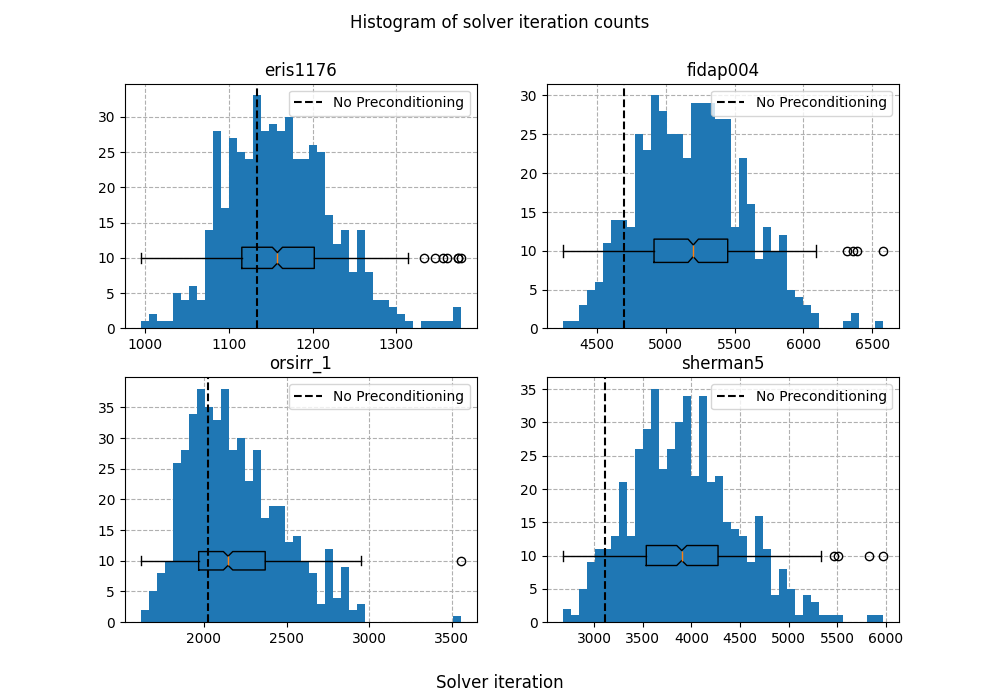
\includegraphics[width=1\textwidth]{plots/initial_par_shift.png}
    \caption{Histogram and boxplot of the solver iterations counts of 500 preconditioned systems for each of the different Matrix Market matrices with a plot for each, with a dashed line corresponding to the unpreconditioned system solver iteration count.}
    \label{fig: initial par shift test}
\end{figure}
\begin{table}[H]
    \center
    \begin{tabular}{|l|r|r|r|r|r|r|}
        \hline
        Matrix & \begin{tabular}{@{}l@{}} Without \\ preconditioning \end{tabular}& Mean & Median & std & \begin{tabular}{@{}l@{}} Number with \\lower iteration count \end{tabular} & Breakdowns\\\hline
        eris1176 & 1134 & 1159.39 & 1157 & 81.85  & 175 & 1\\
        fidap004 & 4695 & 5197.11 & 5200.5 & 384.88 & 47 & 0\\
        orsirr\_1 & 2025 & 2190.75 & 2146 & 287.80 & 163 & 0\\
        sherman5 & 3115 & 3904.15 & 3898.5 & 606.91 & 31 & 5\\\hline
    \end{tabular}
    \caption{Solver iteration count statics of the four matrices preconditioned systems. With each column in order corresponding to the name of the matrix; the solver iteration count for the unpreconditioned system; the mean, median and standard deviation preconditioned solver iteration counts; the number of preconditioned matrices which have a had a solver iteration count lower than the unpreconditioned system; number of preconditioned system that suffered from a breakdown.}
    \label{table: initial par shift stat}
\end{table}
From both the histograms in figure \ref{fig: initial par shift test} and the second to last column of table \ref{table: initial par shift stat}, showing how many of the preconditioned systems had a fewer number of solver iterations, we can see that partitioned shift preconditioner can has the possibility of working as preconditioner given the right coefficients. And that the condition number of the original system plays a part in how well the preconditioner works, as the two matrices with the highest condition number has the fewest number preconditioners that improved the solver iteration count, this a bit unexpected as system with a higher base solve iteration count has larger potential for a improvements. It could also mean that the coefficient generations might have a bad distribution to generate a good preconditioner for these two specific systems. This is where the learning of the preconditioner comes in, because then the initial coefficient should not matter, but only if the initial preconditioner would cause a breakdown of the algorithm to occur.


